\section{Representation Learning Methods}\label{review}
In this chapter any found paper proposing a RL strategy used for time series data with adaptability on AD tasks is presented. For the literature research the inclusion criteria as described in \autoref{criteria} are applied.

The different RL strategies are explained focusing on compliance of the exclusion criteria. The strategies are organized by their underlying concept. First straight-forward methods which are based on one concept are presented and the complexity increases throughout the chapter. In the end combinations of different concepts are presented.
\subsubsection{MLP}
% INRAD
Using a simple MLP is a straight-forward way to learn representations and to detect anomalies in time series data \cite{nielsen_neural_2015}. The input variable for the MLP are time points and the output variable represents the value at these time points. The model is trained to learn this mapping. With the trained model, the values in a live scenario are predicted and the difference to the actual values is measured. If the difference exceeds a certain threshold, an anomaly is found. A method called INRAD, Implicit Neural Representation of time series Data is using this concept. The method takes multiple variables as input and the model is trained with data including anomalies. It is not suitable for ZSL \cite{jeong_time-series_2022}.
\subsubsection{RNN}
\cite{su_robust_2019} propose a method called OmniAnomaly for AD in MVTSD using a Stochastic Recurrent Neural Network to model the temporal dependencies.
The key advantage of this method is its robustness to noisy and high-dimensional data according to the authors. The model learns to represent normal patterns in time series and identifies deviations from these patterns as anomalies. Since OmniAnomaly depends on having access to representative normal data to learn patterns, it is not suitable for zero-shot scenarios.
\subsubsection{CNN}
Methods based on CNNs are normally used for classification of images but in recent papers they are used to detect anomalies in images. \cite{aota_zero-shot_2023} develop a Texture AD and achieve a high performance in ZSL. They compare Zero-Shot against Many-Shot Learning in their work. Several image AD tools can be found (\cite{sabokrou_deep-anomaly__2018}, \cite{aota_zero-shot_2023}). But CNNs perform on time series data as well.

The main idea of using CNNs is to predict a value based on the input frame. If the distance between the predicted and the actual value exceeds a predefined threshold, the anomaly can be detected.

% CyberAttacks Kravchick
This idea is used to detect cyberattacks in industrial control systems. A recent study uses a dataset from a Secure Water Treatment testbed to identify cyber anomalies by measuring the statistical deviation between predicted and observed values. They explore different deep learning architectures, including CNNs and recurrent networks, and find that one dimensional CNNs perform particularly well for time series prediction tasks. Their approach successfully detects the majority of cyber attacks with minimal false positives, highlighting the effectiveness of CNNs in real-time AD in MVTSD \cite{kravchik_detecting_2018}. However, the paper does not discuss the usability on ZSL. In the same area a method detecting unknown cyber-attacks is presented in \cite{zhang_unknown_2020} who use an Autoencoder which is discussed later on.

% TCN
\cite{he_temporal_2019} use Temporal Convolutional Networks (TCN). TCNs restrict the output to be dependent on past and present time steps only. This enables them to capture temporal dependencies. By training on normal patterns, the network learns to predict future values. Significant deviations between these predictions and actual observations indicate potential anomalies. The authors do not mention if the method works in a ZSL scenario but the method only learns normal data, which indicates a usability for ZSL.

% SLMR
Another paper introduces a mask-based self-supervised representation learning approach to extract both short-term local dependencies and long-term global trends. By integrating forecasting and reconstruction-based models, the method effectively captures temporal contexts and feature correlations. An attention mechanism ensures feature importance, leading to better AD performance on various datasets. The method is designed for MVTSD AD but does not explicitly address ZSL scenarios \cite{miao_unsupervised_2022}.

\subsubsection{Contrastive Learning}
% Paper Debiased CL
In \cite{zhang_debiased_2024} a framework using CL is proposed which is applied for industrial fault detection. Two data sets that consist of various vibration signals of industrial machines and stiction sensors with multiple variables are used for training. The effectiveness of the proposed framework is demonstrated through its application to these datasets.

% CARLA
CL is also used for AD of time series in \cite{darban_carla_2024}. They use CL combined with synthetic anomaly injection. CL enables them to capture patterns in time series data and the framework shows good results on common real world datasets according to the authors. Like in the previous paper, dissimilar pairs, the anomalies, build distant data points and similar data points are close to each other. In order to train the model artificial anomalies are injected which build distant pairs. In the next stage the classification is done by the proximity of the neighbours in the representation space. Additionally anchor points representing the nearest and furthest neighbour are given from each representation as seen in \autoref{fig_arch_carla}. An implementation by the authors can be found \footnote{\fussy\tiny github.com/zamanzadeh/CARLA \label{foot_carla}}.
\begin{figure}[h!] % 'h!' tries to place the figure here
  \centering
  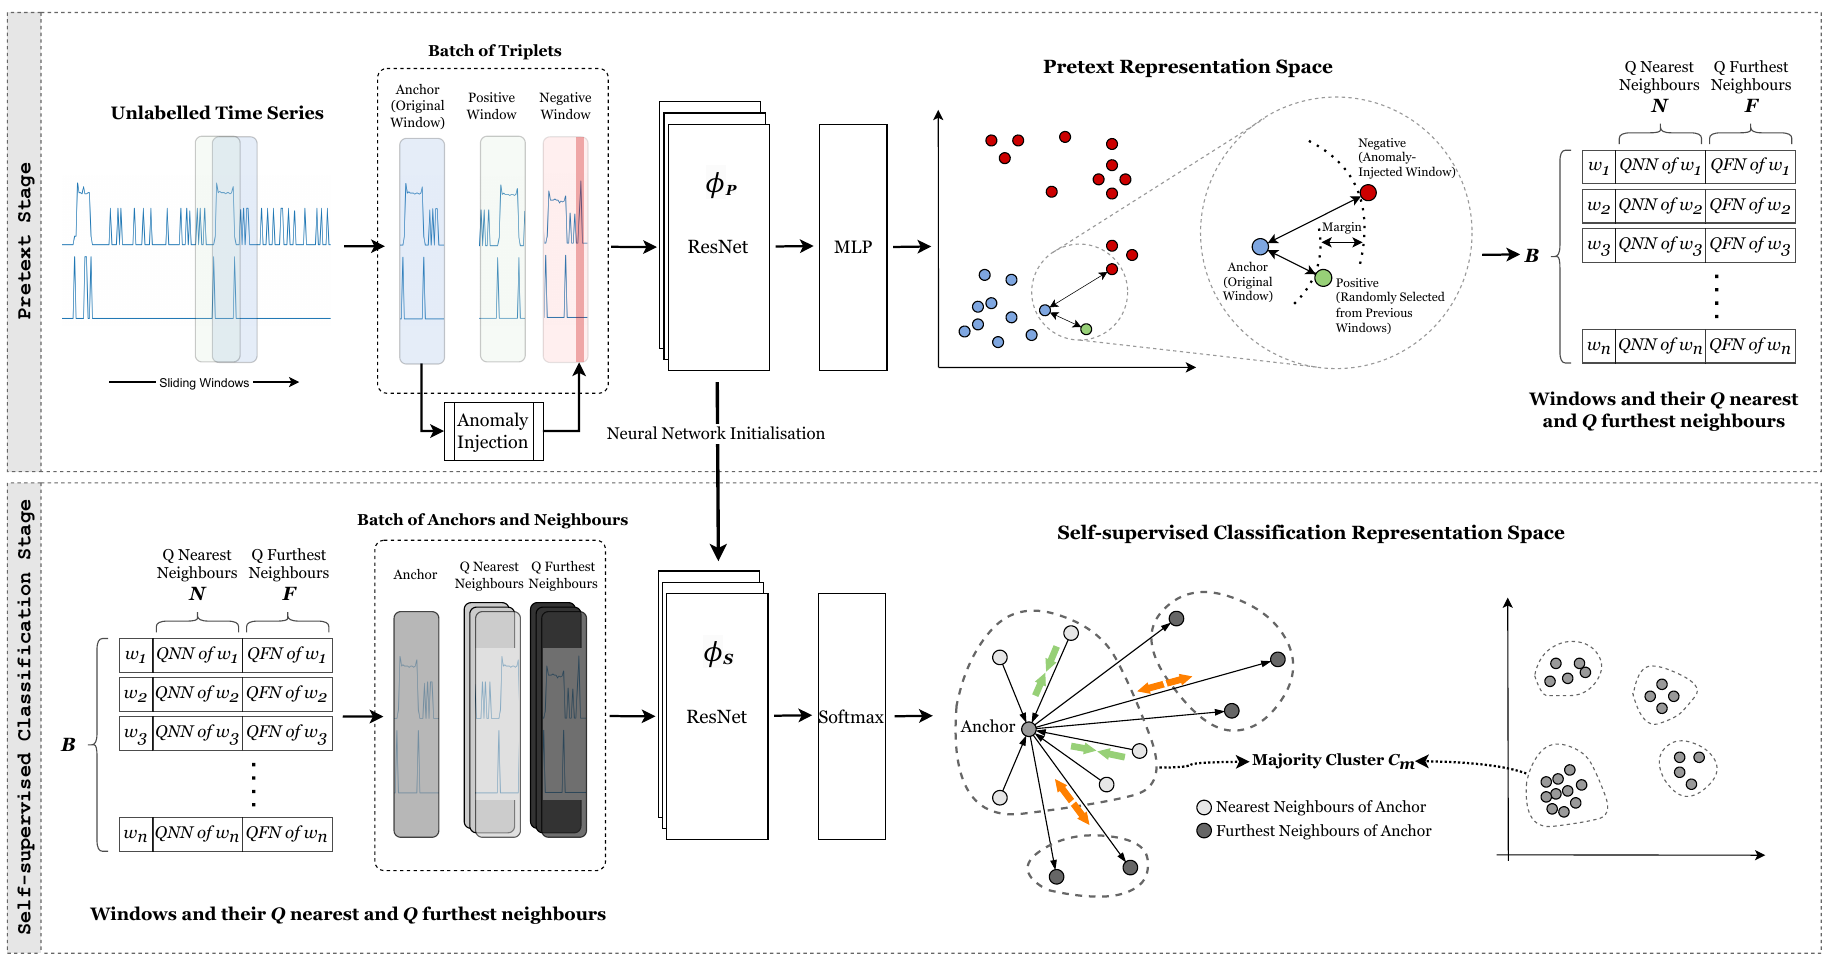
\includegraphics[width=0.8\textwidth]{images/arch_carla.png}
  \caption{Architecture of the method CARLA \cite{darban_carla_2024}}
  \label{fig_arch_carla}
\end{figure}

% CL-TAD
CL-TAD, a method for time series AD that uses CL and reconstruction-based techniques addresses the challenges of temporal dynamics, label scarcity, and data diversity in real-world applications. The method comprises two main components: positive sample generation and contrastive-learning-based representation learning. Positive samples are generated by reconstructing masked parts of the time series data, helping the model learn the underlying normal patterns. These samples, along with the original data, are then fed into a CL framework, which contrasts pairs of similar and dissimilar samples to learn representations \cite{ngu_cl-tad_2023}.
While CL-TAD is not explicitly designed as a ZSL method, its use of CL and reconstruction-based techniques suggests that it could have potential in zero-shot AD scenarios. A tutorial for implementation can be found \footnote{\fussy\tiny github.com/nguhcv/cl-tad/tree/main}.

% OCC based methods
% COCA
To succeed on Zero-Shot AD, One-Class Classification (OCC) can be useful.
By gathering all "normal" values into a single class the outliers are directly detected if they are outside of it.
The COCA (Contrastive One-Class AD) method combines CL with OCC to improve AD in MVTSD. By treating original and reconstructed representations as positive pairs, it optimizes a contrastive one-class loss function that enhances the detection of anomalies while preventing common issues. Although COCA is designed for self-supervised AD, its ability to learn from unlabeled data suggests potential applicability in ZSL scenarios, though this has not been explicitly tested \cite{wang_deep_2023}. An implementation script is provided by the authors \footnote{\fussy\tiny github.com/ruiking04/COCA}.

%
The paper by \cite{lee_time_2023} presents an approach for detecting anomalies also using OCC in industrial time series data, which typically lacks labels for supervised learning. They combine OCC with CL to define a new objective function that can simultaneously learn from both models. This method enhances feature extraction while preserving temporal characteristics. The paper demonstrates the method's effectiveness through high AD performance on datasets with similar normal and anomalous data forms, highlighting its potential in industrial applications.

Unlike traditional OCC methods that map all normal instances into a single hypersphere, the method presented by \cite{chen_time-series_2023} focuses on local contextual information. By pulling each normal instance towards its recent context window, it aims to better detect context-based anomalies. The model uses a deterministic contrastive loss, which improves the network's ability to distinguish between normal and abnormal data. The authors did not test the method in a ZSL scenario and no public implementation can be found.

% TS2Vec
\cite{yue_ts2vec_2022} introduce TS2Vec, a framework for learning robust and universal time series representations at multiple levels through hierarchical CL. TS2Vec captures characteristics of different time series instances and dynamic temporal patterns within each series. The method is tested on ZSL and is applicable for MVTSD. The instructions on reproducing the outcomes are made publicly available by the authors \footnote{\fussy\tiny github.com/zhihanyue/ts2vec \label{foot_ts2vec}}.

% TimeAutoAD
Another paper introduces an autonomous system for AD in MVTSD also using CL. The proposed method TimeAutoAD automates model configuration and hyperparameter optimization. It uses self-supervised CL to enhance the model's ability to differentiate normal and anomalous time series by generating pseudo-negative samples. The method is tested on real-world datasets. The paper does not explicitly address zero-shot AD \cite{jiao_timeautoad_2022}.

% ContrastAD
The ContrastAD framework presented in \cite{li_contrastive_2023} is a self-supervised method for time series AD that leverages CL with temporal transformations. The key innovation is the use of anomaly-induced transformations to create representations that differentiate between normal and abnormal data. This approach targets both point anomalies and contextual anomalies in MVTSD. By learning representations for normal and anomalous data in the latent space, ContrastAD improves performance on noisy and complex datasets. However, the method is not trained or validated on entirely new types of anomalies.

% DCdetector
Another model called DCdetector presented in \cite{yang_dcdetector_2023} is an attention-based CL framework designed for time series AD. It utilizes a dual attention asymmetric design to create a permutation-invariant representation, guiding the learning process. This approach enhances the model's ability to discriminate between normal and anomalous data. Extensive experiments demonstrate that DCdetector achieves state-of-the-art performance across multiple benchmark datasets. While the paper focuses on its effectiveness in AD, it does not explicitly address or test the model's applicability to ZSL scenarios \cite{yang_dcdetector_2023} In the article a repository containing bash scripts for implementation can be found \footnote{\fussy\tiny github.com/DAMO-DI-ML/KDD2023-DCdetector}.

%Contrastive Predictive Coding Methods:
\cite{pranavan_contrastive_2022} presents a novel approach for AD in MVTSD using Contrastive Predictive Coding (CPC). Their method, named time series Representational Learning through Contrastive Predictive Coding (TRL-CPC), aims to capture the temporal dependencies and correlations across multiple variables in time series data.
The TRL-CPC framework consists of an encoder, an auto-regressive model, and a non-linear transformation model. These components are optimized to learn the representations of MVTSD by predicting future segments from past segments. The core idea is to maximize the mutual information between the encoded representations of past and future segments, thereby learning robust representations.
To detect anomalies, TRL-CPC calculates the prediction error between actual future segments and the predicted segments generated by the CPC model. Anomalies are identified where this prediction error exceeds a certain threshold, enabling unsupervised AD based on the structure of the data itself.

% TiCTok
CPC is also used by the method TiCTok presented in \cite{kang_tictok_2023}. The model proposes an approach to MVTSD AD with a time series token encoder. This encoder converts raw time series data into latent embeddings that capture wide-ranging temporal information. The model employs CL to produce representations, which help distinguish between normal and anomalous data. Additionally, TiCTok introduces a new anomaly scoring method based on the contrastive loss used during training. In their paper they do not test the model on ZSL scenarios.

% MGCLAD
Another paper introduces Multiview Graph CL for detecting anomalies in MVTSD, particularly in IoT systems. The method constructs graph structures to model both temporal context and signal dependencies, while an adaptive data augmentation strategy generates graph views for CL. This approach enhances representation quality and improves performance in AD tasks except ZSL \cite{qin_multiview_2023}. The method is available on Github \footnote{\fussy\tiny github.com/shuxin-qin/MGCLAD}.

% TriAD
The paper by \cite{sun_unraveling_2023} introduces TriAD (Tri-domain Anomaly Detector), a self-supervised learning method for time series AD. TriAD models features across three domains: temporal, frequency, and residual. Without relying on labeled anomalies. Unlike traditional CL, TriAD uses inter-domain and intra-domain contrastive losses to learn shared attributes among normal data and distinguish them from anomalies. The approach is designed to handle anomalies of varying lengths and shapes \cite{sun_unraveling_2023}. The authors provide a link to their implementation \footnote{\fussy\tiny github.com/pseudo-Skye/TriAD}.

In summary methods using CL are mostly not tested on ZSL. Their robustness against noisy data is not ensured.

\subsubsection{Autoencoder}
Autoencoders on the other hand are robust to unclean training datasets \cite[p. 2487]{abdulaal_practical_2021}. Due to their architecture noise is filtered from the input.

\cite{provotar_unsupervised_2019} introduces an AD method using an autoencoder architecture based on Long Short-Term Memory (LSTM) networks. The core idea is that an LSTM autoencoder learns to compress and reconstruct the input time series data. During training, the model learns the normal patterns in the data by minimizing the reconstruction error. When fed new data, the model attempts to reconstruct it, and any significant reconstruction error signals an anomaly. This approach is particularly effective because LSTMs are well-suited to capture temporal dependencies, making them ideal for time series data. The model works without requiring labeled datasets, making it an unsupervised solution. The authors test the model on both synthetic and real-world data, such as sound event detection. It can effectively detect outliers based on reconstruction error but does not have the capacity for ZSL.

% LATAM
A method called LATAM (Long short-term memory Autoencoder with Temporal Attention Mechanism) also uses LSTMs for AD in MVTSD. Temporal dependencies are combined with dynamic thresholding, which adapts the threshold throughout the evaluation of the model. They train the model on inverter data including failures and evaluate it on other benchmark datasets explicitly in few-shot scenarios \cite{nivarthi_towards_2023} The source code is provided by the authors \footnote{\fussy\tiny github.com/anonymousgit234/FewShot-Anomaly-Detection-using-LATAM}.

% Other LSTM based
Other methods that use LSTM networks are found in literature. All of them are designed for MVTSD but are not tested on ZSL. The authors did not provide instructions on how to replicate the outcomes
\cite{yokkampon_robust_2022} \cite{gao_tsmae_2023} \cite{niu_lstm-based_2020}.

% MST-VAE
\cite{pham_mst-vae_2022} proposes a Multi-Scale Temporal Variational Autoencoder (MST-VAE) for AD in MVTSD. MST-VAE combines short and long-scale convolutional kernels within a 1D CNN and a Variational Autoencoder to capture both short-term and long-term temporal patterns. The method is not directly tested in a Zero-Shot scenario. An implemention is provided by the authors \footnote{\fussy\tiny github.com/tuananhphamds/MST-VAE}.

% MSCVAE
% Another method using VAE introduces a Multi-Scale Convolutional Variational Autoencoder (MSCVAE) for unsupervised AD in MVTSD. It constructs multi-scale attribute matrices to capture system states at different time steps and uses a convolutional variational autoencoder to extract spatial features, while an attention-based ConvLSTM captures temporal patterns. Anomalies are detected by comparing the original and reconstructed matrices, and a novel ERR-based threshold strategy is employed for optimal performance. The article does not mention ZSL and neither provides an open source implementation .

% VRAE based
To detect anomalies in healthcare data a variational recurrent autoencoder (VRAE) is used in \cite{pereira_learning_2019}. They created an unsupervised framework where the model learns to represent the data and detect anomalies. During training, they add noise to the input data, and the model tries to reconstruct the original, uncorrupted data. This helps the model learn more robust representations of the data. To detect anomalies, they cluster these learned representations and calculate the distance to identify outliers. Their approach was tested on a benchmark electrocardiogram dataset and showed that it could effectively detect unusual heartbeats.

%
Another approach using VRAE involves creating synthetic anomalies to improve the detection process. First, they distill feature descriptors of normal data points into more robust representations using AEs. These representations are then refined using a VAE that creates a family of distributions. From these distributions, they select those that lie on the outskirts of the normal data as generators of synthetic anomalies.
By generating these synthetic anomalies, they train binary classifiers to distinguish between normal and abnormal data. Their hierarchical structure for feature distillation and fusion helps create robust representations, enabling effective AD without needing actual anomalies during training \cite{ramirez_rivera_anomaly_2022}.

% VRQRAE
Kieu et al. propose Variational Quasi-Recurrent Autoencoders (VQRAEs) for unsupervised time series AD, using robust divergences to improve resilience against noisy data. VQRAEs utilize Quasi-Recurrent Neural Networks (QRNNs) for efficient temporal dependency capture, and a bi-directional version (BiVQRAEs) enhances accuracy by processing data in both forward and backward directions. However the method was not explicitly tested on ZSL \cite{kieu_anomaly_2022}. An implementation is provided by the authors \footnote{\fussy\tiny github.com/tungk/Bi-VQRAE}.

% Unknwon CyberAttacks
A previously mentioned paper addresses the challenge of detecting unknown cyberattacks by applying ZSL. The proposed method maps the features of known attacks to a semantic space using a sparse autoencoder and restores them to the feature space by minimizing reconstruction errors. This technique enables the model to detect previously unseen attacks by generalizing from known attack features. The research highlights the feasibility and effectiveness of ZSL for cybersecurity applications \cite{zhang_unknown_2020}.

% FuSAGNet
A method called Fused Sparse Autoencoder and Graph Net (FuSAGNet) is used for AD in MVTSD. The method combines a Sparse Autoencoder (SAE) to learn sparse latent representations and a Graph Neural Network (GNN) to forecast future time series behavior. It captures both temporal dependencies and complex interfeature relationships by learning graph structures from the data. This joint optimization approach aims to improve AD performance by fusing reconstruction and forecasting tasks. The method was empirically tested on three real-world datasets related to industrial systems but not in ZSL scenarios \cite{han_learning_2022} \footnote{\fussy\tiny github.com/sihohan/FuSAGNet}.

% deep AOC
Deep Autoencoding One-Class (AOC), a method for time series AD that combines autoencoder-based reconstruction and one-class classification in a single-stage approach to better capture normal patterns. The method is evaluated on public datasets, outperforming baseline models and proving effective for detecting various types of anomalies in both univariate and MVTSD. However, ZSL is not tested or addressed in the proposed framework \cite{mou_deep_2023} \footnote{\fussy\tiny github.com/alsike22/AOC}.

% RANSynCoders
Another paper presents a method named RANSynCoders for detecting anomalies in asynchronous multivariate time series by combining spectral analysis with autoencoders. This approach improves performance on high-dimensional, asynchronous data by reducing false positives and providing better localization of anomalies. The method in the paper does not specifically mention being tested in zero-shot scenarios \cite{abdulaal_practical_2021}. An implemention of the method is provided by the authors \footnote{\fussy\tiny github.com/eBay/RANSynCoders}.

% TCN-AE
Another proposed method is using a Temporal Convolutional Network Autoencoder (TCN-AE) designed for unsupervised AD in MVTSD. It employs dilated convolutions to capture long-range dependencies and compresses time series into representations using an autoencoder. The method detects anomalies by evaluating reconstruction errors \cite{thill_temporal_2021}. A Repository with a minimal working example can be found provided by the author but no implementation on ZSL is provided \footnote{\fussy\tiny github.com/MarkusThill/bioma-tcn-ae}.

% MEGA
A framework called Multiscale Wavelet Graph AutoEncoder (MEGA) in presented in \cite{wang_multiscale_2023} for AD in multivariate time series. It integrates Discrete Wavelet Transform (DWT) to decompose time series into different frequency components, reconstructing them to highlight anomalies across scales. Additionally, a dynamic graph convolution network is employed to model inter-variable relationships at different scales, enhancing the detection of anomalies caused by changes in variable dependencies.
This method is tested in a zero-shot scenario and explicitly takes multivariate time series as input. The code is provided by the authors \footnote{\fussy\tiny github.com/jingwang2020/MEGA \label{foot_mega}}.

% DAEMON
The method proposed in \cite{chen_adversarial_2023} introduces DAEMON, an adversarial autoencoder framework designed for unsupervised multivariate time series AD and interpretation. The model employs two training processes: one to align the hidden variable’s posterior distribution with a prior and another to minimize the difference between original and reconstructed data. This improves robustness and avoids overfitting while anomalies are detected based on reconstruction errors. There is no mentioning of testing in a zero-shot scenario.
The authors of the method DAEMON published python scripts for replicating the results on all datasets they used \footnote{\fussy\tiny github.com/Sherlock-C/DAEMON \label{foot_daemon}}.

% GRU-AE
The method proposed in \cite{gong_autoencoder-based_2022} utilizes a Gated Recurrent Unit-based Autoencoder (GRU-AE) to detect anomalies in time series data by reconstructing sequences and identifying large reconstruction errors as anomalies. It incorporates an attention mechanism to enhance performance and applies multi-timestamp stacking to reduce time steps for better training efficiency. The model is tested on real-world datasets from cellular networks, detecting anomalies at both single-day and multi-day scales. The method is applied to MVTSD, but no mention of a zero-shot scenario is made.

%
The method proposed in \cite{wang_attention-based_2022} presents an attention-based encoder-decoder network for AD in time series data, which focuses on learning representations in both seperate feature spaces without needing reconstruction. The attention mechanism is applied to rescale convolutional layers, highlighting the most contributive segments of the data for better representation learning. This approach improves AD by calculating belief scores in both spaces using kernel density estimation (KDE). The method is tested on multivariate time series and in a zero-shot scenario, specifically for detecting new faults but no implementation is provided by the authors.

% MOMENT
To overcome the challenge of poorly available time series data sets \cite{ma_survey_2023}, the model family MOMENT tries to learn general patterns on a pile of time series data following the architecture in \autoref{fig_arch_moment}. The pile is a collection of different datasets which they assembled for their pretraining. According to the paper minimal finetuning is needed to perform on multivariate time series tasks like AD. They published the model and made the usage easily accessible with its own python library \footnote{\fussy\tiny github.com/moment-timeseries-foundation-model/moment/blob/main/tutorials/anomaly\_detection.ipynb \label{foot_moment}}.
The time series datasets the model is trained on consist of domains including weather measurements, sensor values and power consumption datasets. They also included tongue and finger movement of humans. The different tasks which the model is evaluated on are forecasting (long and short horizon), classification, AD and imputation. Except for short-horizon forecasting all tasks are managed well. However it cannot detect anomalies in vertically shifted time series \cite{goswami_moment_2024}.
\begin{figure}[h!] % 'h!' tries to place the figure here
  \centering
  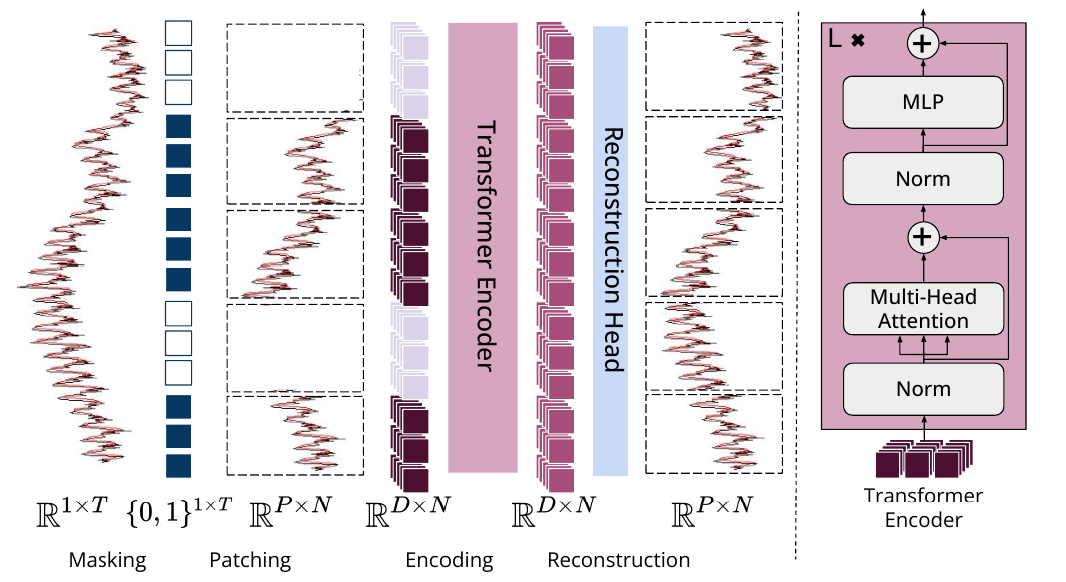
\includegraphics[width=0.8\textwidth]{images/arch_moment.png}
  \caption{Architecture of the method MOMENT \cite{goswami_moment_2024}}
  \label{fig_arch_moment}
\end{figure}


A variety of methods based on AEs can be found. But AE-based methods have remaining challenges. AEs are able to detect anomalies in general but they cannot identify the type of faulty samples \cite{zhang_debiased_2024}.

\subsubsection{Transformer}
Transformers on the other hand, learn the dependence of time points instead of reconstructing the input. This can possibly lead to representations that hold information about the shape of the anomalies.

% AnomalyTransformer
A method called "Anomaly Transformer", which detects anomalies in time series by comparing a time point’s learned associations with a Gaussian-based prior association to compute a Association Discrepancy. The model uses a minimax strategy to amplify the difference between normal and anomalous points based on this discrepancy. The method is not tested in a zero-shot scenario but supports multivariate time series as input \cite{xu_anomaly_2022} \footnote{\fussy\tiny github.com/thuml/Anomaly-Transformer}.

%TranAD
TranAD is a transformer-based model designed for AD in MVTSD. It uses an adversarial training to enhance both accuracy and training stability. The paper does not explicitly mention testing the method in a ZSL scenario \cite{tuli_tranad_2022} \footnote{\fussy\tiny github.com/imperial-quore/TranAD}.

% DATN
A proposed method, Decompose Auto-Transformer Network (DATN), focuses on time series AD by decomposing the input into seasonal and trend components, followed by an auto-attention mechanism for feature extraction. The method takes multivariate input, where the decomposition and attention mechanisms operate on MVTSD. The paper does not mention ZSL explicitly \cite{wu_decompose_2023}.

% TiSAT
Time Series Anomaly Transformer (TiSAT), introduces a transformer-based approach that captures long-range temporal dependencies in time series AD using a probabilistic attention mechanism, which improves computational efficiency by focusing on key query-value pairs. The model takes multivariate input but the authors do not mention ZSL \cite{doshi_tisat_2022} \footnote{\fussy\tiny github.com/kevaldoshi17/TiSAT}.

% TCF-Trans
The TCF-Trans method enhances AD in MVTSD by using a feature fusion decoder that combines shallow and deep layers to capture important anomaly details while resisting noise. It also introduces a temporal context fusion module to adaptively merge predictions for more robust results. Although the method was tested on various datasets, it is not explicitly evaluated in a strict zero-shot scenario \cite{peng_tcf-trans_2023}.

% DCT-GAN
The DCT-GAN method proposed in \cite{li_dct-gan_2023} integrates Dilated Convolutional Networks with Transformers within a GAN framework to enhance the detection of anomalies in time series data, improving generalization and accuracy. There is no specific mention in the document about testing the method on ZSL tasks.

% AnoFormer
The AnoFormer method is a Transformer-based GAN framework for unsupervised multivariate time series AD, utilizing a two-step masking strategy to improve normal data representation and AD. The model masks parts of the data randomly, then remasks uncertain regions based on entropy to refine its focus. While the method excels in unsupervised learning, it is not explicitly tested in a ZSL scenario \cite{shin_time_2023}.

% LLM
A method detecting anomalies in tabular data using Large Language Models (LLM) is presented in \cite{li_anomaly_2024}. In order to perform tasks that LLMs are not directly build for they generate synthetic datasets. Using these datasets LLMs and specifically GPT-4 have comparable performance with transductive learning methods \cite[p. 6]{li_anomaly_2024}. Concerning different batches, the method is tested in ZSL. The model is trained on some batches and evaluated on new ones. Due to the fact that the prompt contains data of one variable, the method is not used for multivariate time series.

% LLMs in general
\cite{su_large_2024} examine a literature review on how LLMs perform on anomaly detection tasks concerning time series data. LLMs in anomaly detection are specifically useful when the time series data is in the form of words. This can be the case in log analysis. Logs are generated over time and hold a lot of information which can detect errors and system failures. They conclude that LLMs have potential in detecting anomalies but challenges remain. The occurrence of hallucinations and the need for computational efficiency to name a few.

% Fourier
Using Fourier Analysis and the transformer architecture is emplloyed in  \cite{ye_multivariate_2023} to detect anomalies in time series data. The encoder of a transformer is used to capture temporal features of time series. They detect frequencies by using Fourier Analysis.

\subsubsection{Shapelet Learning}
% Shapelets: Shapelets are short, representative subsequences extracted from time series data.
% Shapelet Learning: Extraction, Evaluation and Selection of shapelets. Medling
\cite{beggel_time_2019} address the problem of detecting anomalies in time series data using a novel unsupervised method based on shapelet learning. Their method learns representative features that describe the shape of time series data from the normal class and simultaneously learns to accurately detect anomalies. The objective function encourages the learning of a feature representation in which normal time series lie within a compact hypersphere, while anomalous observations lie outside the decision boundary.
The advantage of their approach is that it can efficiently detect anomalies in unseen test data without retraining the model, by reusing the learned feature representation. Experimental results on multiple benchmark datasets demonstrate the robustness and reliability of the method in detecting anomalous time series. They suggest to extend their method on multivariate time series in future works.

% Alshaer
In contrast, \cite{alshaer_detecting_2020} propose a method combining matrix profiles with shapelet learning to handle streaming time series data. The matrix profile efficiently identifies potential anomalies in real-time, and shapelet learning characterizes these anomalies. This approach is particularly suited for environments requiring immediate AD. The authors provide code examples for implementation in their paper but further open source repositories were not found. As the previous work they didn't use the method for multivariate time series and suggest expanding the method for this.

%IPS
The IPS (Instance Profile for Shapelet Discovery) method addresses time series classification by using shapelets-discriminative subsequences of time series. This method was tested extensively on various datasets but was not explicitly tested in a zero-shot scenario \cite{li_ips_2022}.

% SL based
The method proposed in \cite{liang_shapelet-based_2024} focuses on using shapelet-based representations for unsupervised learning of multivariate time series. It employs CL, multi-scale alignment, and a shapelet transformer. The method was tested in scenarios where labeled data is sparse or unavailable, but it does not appear to be tested explicitly in a traditional zero-shot setting \footnote{\fussy\tiny github.com/real2fish/CSL}.

\subsubsection{Combinations}
% Clustering
\cite{li_clustering-based_2021} propose a method for detecting anomalies in multivariate time series by combining clustering and reconstruction techniques. The authors use a sliding window approach to generate subsequences from the multivariate time series, then apply extended fuzzy clustering to reveal the underlying structure of the subsequences. By reconstructing these subsequences with optimal cluster centers, the method detects anomalies based on how well the reconstructed data fits the original subsequences. A confidence index quantifies the level of detected anomalies. The method does not seem to have been explicitly tested in a ZSL scenario.

% Moving Memory Dynamic Filter
A Fourier transformation isolates seasonal components in a method called Moving Memory Dynamic Filter (MMDF). While the distance transformation captures both the data values and their temporal dependencies. Anomalies are detected when the center-to-center distance exceeds the threshold. The authors primarily discuss the proposed method in the context of univariate time series AD and do not explicitly mention its applicability to MVTSD \cite{duan_unsupervised_2021}.

%DCFF-MTAD
In contrast, the method DCFF-MTAD, a multivariate time series AD method uses a dual-channel feature extraction that combines spatial short-time Fourier transformation for spatial features and a graph attention network for temporal features. These features are then fused using a Gated Recurrent Unit for robust AD. The method is not tested on ZSL and is not available as open source \cite{xu_dcff-mtad_2023}.
